\chapter{Message Passing
(Belief Propagation)}\label{ch-mp}


Belief Propagation
was first proposed in 1982
Ref.\cite{pearl1982reverend} by Judea Pearl
to simplify
the exact evaluation of the probability
of one node conditioned 
on other nodes
of a bnet (exact inference).
It gives exact results for trees and
polytrees (i.e. bnets with
a single connected component and
 no
loops). For bnets with loops,
it gives approximate results
(loopy belief propagation),
and it has been generalized to
the junction tree algorithm
(see Chapter \ref{ch-junc-tree})
which can do exact inference
for general bnets with loops.
The basic idea behind
the junction tree algorithm
is to eliminate
loops by clustering
them into single nodes.

In his book Ref.\cite{pearl-1988book},
Pearl explains two types 
of Message Passing (i.e., distributed 
computing in a bnet). In Chapter 4, he discusses
one type of MP which he calls Belief Propagation (BP)
or Belief Updating. In Chapter 5, he introduces
a second type of MP which is he calls Belief Revision, but
which I prefer to call
Explanation Optimization (EO).
This chapter will be devoted to BP only.

This chapter is mostly
based on chapter 4 of 
Ref.\cite{pearl-1988book}
by Pearl.
Refs.\cite{wiki-mp},
and \cite{neapolitan2004learning}
were also helpful in writing this chapter.

\section{Distributed Soldier Counting}
Consider
a group of soldiers marching single file.
Fig.\ref{fig-soldiers}
shows several methods by which 
a member of the group 
can obtain a count 
of the soldiers without
breaking the line to do 
global operations.
This can be done in
a distributed fashion, 
with every soldier doing
only local operations
(i.e.,
each soldier 
can only 
send
messages
to either
the soldier in front
or the one in
back).
Such 
distributed soldier counting is a rudimentary
type of BP.
In the next section,
we will
generalize this BP for soldiers
to BP for a Markov chain.
\newpage


\begin{figure}[h!]
\centering
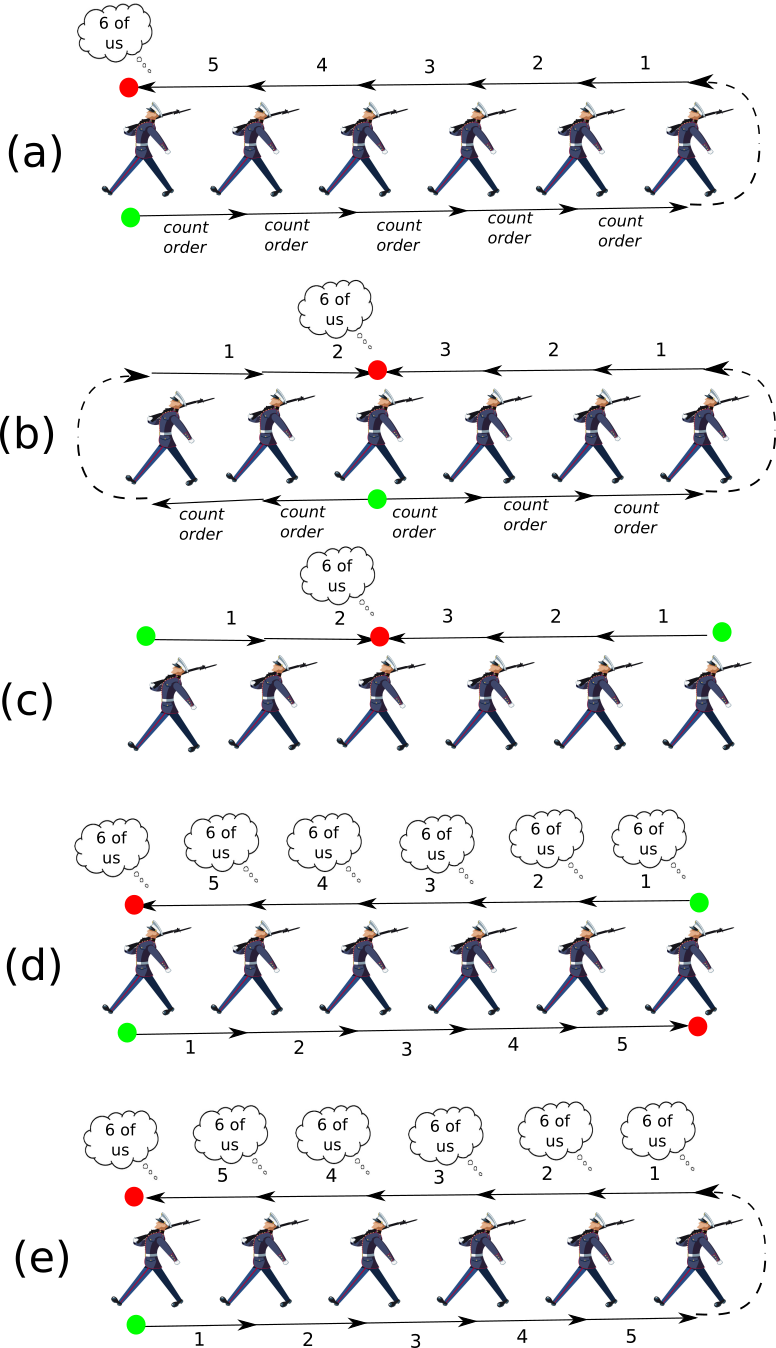
\includegraphics[width=4in]
{mpass/soldiers.png}
\caption{Distributed soldier counting 
(This example
comes from Chapter 4 of
Ref.\cite{pearl-1988book}). 
Green dots indicate the
beginning and red dots the end
of a count. Only
first soldier can calculate
total count in (a). Only 
third soldier can calculate total count
in (b,c). 
All soldiers can calculate
the total count in 
(d,e). One starting point
in (a,b,e).
Two ends as starting points
in (c,d).
} 
\label{fig-soldiers}
\end{figure}

\section{Spring Systems}

\begin{figure}[h!]
\centering
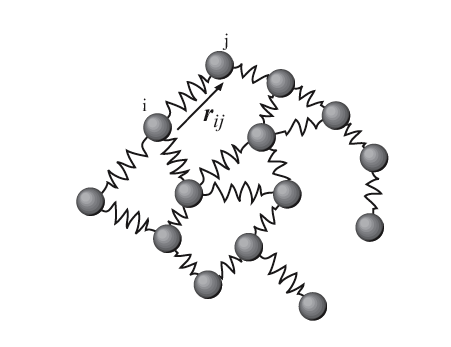
\includegraphics[width=3in]
{mpass/spring-net.png}
\caption{Spring system.
Point masses connected by springs.} 
\label{fig-sping-net}
\end{figure}

See Ref.\cite{wiki-spring-net}
for an introduction to spring systems.
Ideal springs between the point mass
nodes would
not be sufficient.
One would have to add damping to
the springs so as
to reach an equilibrium. 
Time dependent forces (loads)
pointing into or out of the page, applied
to the point masses, would
generate signals that would
propagate 
like BP messages.



\section{BP for Markov Chains}
\begin{figure}[h!]
$$\xymatrix{
\rveps^+
\ar@{<--}@<2ex>[rr]^{\pi_{\rveps^+\ldart\rvx}}
\ar@{.>}@<-2ex>[rr]_{\lam_{\rveps^+\rdart\rvx}}
&&
\rvx\ar[ll]
\ar@{<--}@<2ex>[rr]^{\pi_{\rvx\ldart\rveps^-}}
\ar@{.>}@<-2ex>[rr]_{\lam_{\rvx\rdart\rveps^-}}
&&
\rveps^-\ar[ll]
}$$
\caption{3 node Markov chain
$\rveps^+\larrow\rvx\larrow \rveps^-$.
The $\pi$  messages
(probability functions)
travel downstream (i.e., 
they carry info
in the direction
of the graph arrows, towards the future)
and are indicated by a dashed arrow
or by a left double arrow $\ldart$. 
The $\lam$  messages 
(likelihood functions) travel 
upstream (i.e., they 
carry info opposite to 
direction of the graph arrows,
towards the past)
and are indicated
by a dotted arrow
or by a right double arrow $\rdart$.
$\rveps^+$
stands for future evidence and 
$\rveps^-$ for past evidence. 
}
\label{fig-mp-3chain}
\end{figure}

Consider the 
3 node Markov chain
$\rveps^+\larrow\rvx\larrow \rveps^-$
shown in 
Fig.\ref{fig-mp-3chain}.
Define\footnote{The pattern
behind these definitions,
in case it eludes you, 
is as follows: the $\pi$'s
always carry information
about the past
and the $\lam$'s 
about the future.
But the past or future of 
what? Of the argument
of the function.
Out  of the
two random variables
in the subscript
of the function,
the one on the 
right hand side
of the subscript, 
the  one which
is adjacent but beneath 
 the argument, is always the 
argument.}


\beq
\pi_{\rveps^+\ldart \rvx}(x)=
P(x|\eps^-)
\text{ (past of $\rvx$)}
\eeq

\beq 
\lam_{\rveps^+\rdart \rvx}(x)=
P(\eps^+|x)
\text{ (future of $\rvx$)}
\eeq

\beq
\pi_{\rvx\ldart \rveps^-}(\eps^-)=
P(\eps^-)=\delta(\eps^-, \eps^-_0)
\text{ (past of $\rveps^-$)}
\eeq

\beq 
\lam_{\rvx\rdart \rveps^-}(\eps^-)=
P(\eps^+|\eps^-)
\text{ (future of $\rveps^-$)}
\;.
\eeq
Furthermore,
define the Belief BEL
in $x$
to be 

\beq
BEL_\rvx(x)
=
P(x|\eps)
\;,
\eeq
where

\beq
\rveps=\rveps^+\cup\rveps^-
\;.
\eeq
It follows that

\beqa
BEL_\rvx(x)
&=&
P(x|\eps^+, \eps^-)=
\\
&=&
\caln(!x)
P(\eps^+, x,\eps^-)
\\
&=&
\caln(!x)
P(\eps^+|x)P(x|\eps^-)
\\
&=&
\caln(!x)
\lam_{\rveps^+\rdart \rvx}(x)
\pi_{\rveps^+\ldart \rvx}(x)
\label{eq-2-sided-bayes}
\;.
\eeqa
Note that Bayes rule would affirm
 that\footnote{As usual in this book,
$\caln(!x)$ means
a constant that is independent of $x$.}

\beq
P(x|\eps^+)=
\caln(!x)
\underbrace{P(\eps^+|x)}_
{\lam_{\rveps^+\rdart \rvx}(x)}
P(x)
\;.
\eeq
Thus, Eq.(\ref{eq-2-sided-bayes})
is like a 2-sided Janus Bayes rule.

Note that the $\pi$ messages and
$\lam$ messages propagate 
independently
of each other, via the 
 TPM $P(x|\eps^-)$:

\begin{subequations}
\beq
\underbrace{\pi_{\rveps^+\ldart\rvx}(x)}_
{P(x|\eps^-_0)}
=\sum_{\eps^-}P(x|\eps^-)
\underbrace{\pi_{\rvx\ldart \rveps^-}(\eps^-)}_
{\delta(\eps^-, \eps^-_0)}
\eeq

\beq
\underbrace{
\lam_{\rvx\rdart \rveps^-}(\eps^-)}_
{P(\eps^+|\eps^-)}
=
\sum_x P(x|\eps^-)
\underbrace{
\lam_{\rveps^+\rdart \rvx}(x)}_
{P(\eps^+|x)}
\eeq
\label{eq-pi-lam-propagate}
\end{subequations}

Eqs.(\ref{eq-pi-lam-propagate})
suggest that we define an edge bnet
for the $\pi$ and $\lam$
messages (these messages
live in the edges
between the nodes
$\rveps^+, \rvx, \rveps^-$).
Such an edge bnet, shown
in Fig.\ref{fig-BEL-2pi}, is 
complementary to 
bnet for the nodes themselves.
We will call it
the {\bf BP 2-track bnet}
for the bnet Fig.\ref{fig-mp-3chain},
because it has two ``tracks",
one for $\pi$ messages and another
for $\lam$ ones.
The TPMs, shown in blue,
for the nodes of bnet
Fig.\ref{fig-BEL-2pi}, are 
as follows:

\begin{figure}[h!]
$$\xymatrix{
&\ul{\pi}_{\rveps^+\ldart\rvx}\ar[dr]
&&\ul{\pi}_{\rvx\ldart\rveps^-}\ar[ll]
\\
&&\rvB_\rvx
\\
&\ul{\lam}_{\rveps^+\rdart\rvx}\ar[rr]\ar[ru]
&&\ul{\lam}_{\rvx\rdart\rveps^-}
}$$
\caption{BP 2-track
bnet for the bnet
 Fig.\ref{fig-mp-3chain}.}
\label{fig-BEL-2pi}
\end{figure}

\beq\color{blue}
P(\pi_{\rvx\ldart \rveps^-})= 
\prod_{\eps^-}
\indi(\pi_{\rvx\ldart \rveps^-}(\eps^-)
=P(\eps^-))
\eeq

\beq\color{blue}
P(\pi_{\rveps^+\ldart \rvx}|
\pi_{\rvx\ldart \rveps^-})=
\prod_x
\indi\left(
\pi_{\rveps^+\ldart \rvx}(x)=
\sum_{\eps^-}P(x|\eps^-)
\pi_{\rvx\ldart \rveps^-}(\eps^-)
\right)
\eeq

\beq\color{blue}
P(B_\rvx|
\pi_{\rveps^+\ldart \rvx},
\lam_{\rveps^+\rdart \rvx})=
\prod_x
\indi\left(
B_\rvx(x)=BEL_\rvx(x)
\right)
\eeq

\beq\color{blue}
P(
\lam_{\rveps^+\rdart \rvx})=
\prod_{x}
\indi\left(
\lam_{\rveps^+\rdart \rvx}(x)
=
P(\eps^+|x)
\right)
\eeq

\beq\color{blue}
P(\lam_{\rvx\rdart \rveps^-}|
\lam_{\rveps^+\rdart \rvx})=
\prod_{\eps^-}
\indi\left(
\lam_{\rvx\rdart \rveps^-}(\eps^-)
=
\sum_x P(x|\eps^-)
\lam_{\rveps^+\rdart \rvx}(x)
\right)
\eeq

\hrule

\begin{figure}[h!]
$$\xymatrix{
\rveps^+
\ar@{<--}@<2ex>[rr]^{\pi_{\rveps^+\ldart\rvb}}
\ar@{.>}@<-2ex>[rr]_{\lam_{\rveps^+\rdart\rvb}}
&&
\rvb\ar[ll]
\ar@{<--}@<2ex>[rr]^{\pi_{\rvb\ldart\rvx}}
\ar@{.>}@<-2ex>[rr]_{\lam_{\rvb\rdart\rvx}}
&&
\rvx\ar[ll]
\ar@{<--}@<2ex>[rr]^{\pi_{\rvx\ldart\rva}}
\ar@{.>}@<-2ex>[rr]_{\lam_{\rvx\rdart\rva}}
&&
\rva\ar[ll]
\ar@{<--}@<2ex>[rr]^{\pi_{\rva\ldart\rveps^-}}
\ar@{.>}@<-2ex>[rr]_{\lam_{\rva\rdart\rveps^-}}
&&
\rveps^-\ar[ll]
}$$
\caption{5 node Markov chain}
\label{fig-mp-5chain}
\end{figure}

So far in 
this section, we have considered Markov
chains with 3 nodes.
Before 
concluding our
discussion of BP for Markov chains,
let us consider BP
for a slightly longer chain.
Let us consider
the 5 node Markov
chain
$\rveps^+\larrow\rvb\larrow\rvx\larrow\rva\larrow\rveps^-$
shown in Fig.\ref{fig-mp-5chain}.
We have already dealt 
with the end nodes
of a Markov chain in the 
3 node Markov chain
example above,
so in the 
5 node case, let us
focus on the internal (i.e., not at
an end) node $\rvx$ and its neighbors
$\rva$ and $\rvb$. Define



\beq
\pi_{\rvb\ldart \rvx}(x)=
P(x|\eps^-)
\text{ (past of $\rvx$)}
\;,
\eeq

\beq 
\lam_{\rvb\rdart \rvx}(x)=
P(\eps^+|x)
\text{ (future of $\rvx$)}
\;,
\eeq

\beq
\pi_{\rvx\ldart \rva}(a)=
P(a|\eps^-)
\text{ (past of $\rva$)}
\;
\eeq
and

\beq 
\lam_{\rvx\rdart \rva}(a)=
P(\eps^+|a)
\text{ (future of $\rva$)}
\;.
\eeq
Define the Belief BEL in $x$ to be

\beq
BEL_\rvx(x)
=
P(x|\eps)
\;,
\eeq
where

\beq
\rveps=\rveps^+\cup\rveps^-
\;.
\eeq
Then


\beqa
BEL_\rvx(x)
&=&
\caln(!x)
P(\eps^+|x)P(x|\eps^-)
\\
&=&
\caln(!x)
\lam_{\rvb\rdart \rvx}(x)
\pi_{\rvb\ldart \rvx}(x)
\;.
\eeqa

In analogy
with the case of BP for a 3 node Markov
chain, we can define the bnet
Fig.\ref{fig-BEL-4pi},
which we refer to as the
{\bf BP
2-track bnet} for Fig.\ref{fig-mp-5chain}.
The TPMs, printed in blue,
 for the 
nodes of bnet Fig.\ref{fig-BEL-4pi}, are
as follows:





\begin{figure}[h!]
$$\xymatrix{
&\ul{\pi}_{\rveps^+\ldart\rvb}\ar[dr]
&&\ul{\pi}_{\rvb\ldart\rvx}\ar[ll]\ar@[red][dr]
&&\ul{\pi}_{\rvx\ldart\rva}\ar@[red][ll]\ar[dr]
&&\ul{\pi}_{\rva\ldart\rveps^-}\ar[ll]
\\
&&\rvB_\rvb
&&\rvB_\rvx
&&\rvB_\rva
\\
&\ul{\lam}_{\rveps^+\rdart\rvb}\ar[rr]\ar[ur]
&&\ul{\lam}_{\rvb\rdart\rvx}\ar@[red][rr]\ar@[red][ur]
&&\ul{\lam}_{\rvx\rdart\rva}\ar[rr]\ar[ur]
&&\ul{\lam}_{\rva\rdart\rveps^-}
}$$
\caption{BP 2-track bnet for the bnet
Fig.\ref{fig-mp-5chain}.}
\label{fig-BEL-4pi}
\end{figure}


\beq\color{blue}
P(\pi_{\rvb\ldart\rvx}|\pi_{\rvx\ldart\rva})=
\prod_{x}\indi\left(
\pi_{\rvb\ldart\rvx}(x)=\sum_a P(x|a)
\pi_{\rvx\ldart\rva}(a)
\right)
\label{eq-pr-pi-bar-pi}
\eeq

\beq\color{blue}
P(B_\rvx|
\pi_{\rvb\ldart \rvx},
\lam_{\rvb\rdart \rvx})=
\prod_x
\indi\left(
B_\rvx(x)=BEL_\rvx(x)
\right)
\eeq

\beq\color{blue}
P(\lam_{\rvx\rdart \rva}|
\lam_{\rvb\rdart \rvx})=
\prod_{a}
\indi\left(
\lam_{\rvx\rdart \rva}(a)
=
\sum_x P(x|a)
\lam_{\rvb\rdart \rvx}(x)
\right)
\label{eq-pr-lam-bar-lam}
\eeq

Let us represent the Markov
chain of Fig.\ref{fig-mp-5chain}
by
$\rvx_{nx-1}
\larrow \ldots, \rvx_2\larrow \rvx_1\larrow \rvx_0$
where $nx=5$.
For any node 
$\rvx_i$
with
parent $\ul{px}_i=\rvx_{i-1}$
and child $\ul{cx}_i=\rvx_{i+1}$, 
define
the {\bf memory matrix}
$\calm_{\rvx_i}$
for node $\rvx_i$
as

\beq
\calm_{\rvx_i}=
[
\calm^+_{\rvx_i},
\calm^-_{\rvx_i}]
\;,
\eeq
where $+=$future, $-=$past, and 

\beq
\calm^+_{ \rvx_i}=
\left[
\begin{array}{c}
\pi_{\ul{cx}_i\ldart \rvx_i}(\cdot)
\\
\lam_{\ul{cx}_i\rdart \rvx_i}(\cdot)
\end{array}
\right]
\;, 
\;\;\;
\calm^-_{\rvx_i}=
\left[
\begin{array}{c}
\pi_{\rvx_i \ldart \ul{px}_i}(\cdot)
\\
\lam_{\rvx_i \rdart \ul{px}_i}(\cdot)
\end{array}
\right]
\;.
\eeq 
Note that

\beq
\calm^-_{\rvx_i}=
\calm^+_{\ul{px}_i}
\label{eq-mem-overlap}
\eeq
for all nodes $\rvx_i$.
We will refer to
Eqs.(\ref{eq-mem-overlap}) as
the {\bf memory overlap
conditions}.

We will also use a permuted version of the 
memory matrix

\beq
\calm'_{\rvx_i}=
[
\calm^{OUT}_{\rvx_i},
\calm^{IN}_{\rvx_i}]
\;,
\eeq
where

\beq
\calm^{OUT}_{ \rvx_i}=
\left[
\begin{array}{c}
\pi_{\ul{cx}_i\ldart \rvx_i}(\cdot)
\\
\lam_{\rvx_i \rdart \ul{px}_i}(\cdot)
\end{array}
\right]
\;, 
\;\;\;
\calm^{IN}_{\rvx_i}=
\left[
\begin{array}{c}
\pi_{\rvx_i \ldart \ul{px}_i}(\cdot)
\\
\lam_{\ul{cx}_i\rdart \rvx_i}(\cdot)
\end{array}
\right]
\;.
\eeq

\begin{figure}[h!]
$$\xymatrix{
\ucalm_{\rveps^+}
&
\ucalm_\rvb\ar[l]
&
\ucalm_\rvx\ar[l]
&
\ucalm_\rva\ar[l]
&
\calm_{\rveps^-}\ar[l]
}$$
\caption{BP Memory Bnet for the bnet
Fig.\ref{fig-mp-5chain}. }
\label{fig-mem-5chain}
\end{figure}

Unfortunately,
2-track bnets cannot be
 generalized in any
obvious way  from 
Markov chains to more
complicated DAGs.
An alternative to 2-track bnets
that still
carries message
info in its nodes,
are memory bnets. An BP
{\bf memory bnet}
is a bnet 
which takes each node
of an original
bnet and
adds a local memory to it.
More specifically,
it keeps tha DAG
but replaces each node
$\rvx_i$
by a memory $\ucalm_{\rvx_i}$.
Fig.\ref{fig-mem-5chain} shows 
the memory bnet for
the bnet Fig.\ref{fig-mp-5chain}.
The TPM, printed in blue,
for the  node $\ucalm_\rvx$
of the memory bnet 
Fig.\ref{fig-mem-5chain}, is as follows

\beq\color{blue}
P(\calm_{\rvx_i}|
\calm_{\rvn\in nb(\rvx_i)}
)= A B
\;,
\eeq
where

\beq
A=
\indi(\calm^{-}_{\rvx_i}=\calm^{+}_{\ul{px}_i})
\;,
\eeq
and

\beq
B=
\indi(\calm^{OUT}_{\rvx_i}=\calc(\calm^{IN}_{\rvx_i}))
\label{eq-mp-update-static}
\;.
\eeq
The function $\calc$,
which 
we will call the {\bf BP local computation},
maps $\calm^{IN}_{\rvx_i}$
into $\calm^{OUT}_{\rvx_i}$. More explicitly,
$\calc$ is defined so that

\beq
B
=
\underbrace{P(\pi_{\rvb\ldart\rvx}|
\pi_{\rvx\ldart\rva})}_{B_\pi}
\underbrace{P(\lam_{\rvx\rdart \rva}|
\lam_{\rvb\rdart \rvx})}_{B_\pi}
\;,
\eeq
where
$B_\pi$ and $B_\lam$
are given by Eqs.(\ref{eq-pr-pi-bar-pi})
and (\ref{eq-pr-lam-bar-lam}),
respectively.



The BP memory bnet
 Fig.
\ref{fig-mem-5chain}
is a deterministic bnet.
A deterministic bnet
is basically
just a coupled system
of equations (CSE)
for some unknowns $x_i$. 
A CSE per se does not
include with it a method for  
solving for the $x_i$. Such methods are not
unique.
For example,
for the 
distributed
soldier counting 
problem,
the various 
methods that
we described
for counting soldiers
are just different
methods 
for solving the same
CSE.
One can describe 
a method for solving a
CSE using a dynamic
bnet.\footnote{
The term
dynamic bnet
was used in Chapter \ref{ch-dyn-bnet}
to mean a time inhomogeneous
Markov chain, but 
here we are stretching its meaning to
include
Markov chains
that aren't 
time inhomogeneous.}
To solve
the CSE
represented by
the memory bnet Fig.\ref{fig-mem-5chain},
we will use the 
dynamic bnet 
Fig.\ref{fig-propagation-5chain}.
Henceforth, 
we will refer to
Fig.\ref{fig-propagation-5chain} as
an {\bf BP dynamic bnet}
for Fig.\ref{fig-mem-5chain}.

\begin{figure}
$$\xymatrix{
\rveps^-\ar[d]
&\ucalm^{(0)}_{\rveps^-}\ar[r]\ar[dr]
&\ucalm^{(1)}_{\rveps^-}\ar[r]
&\ucalm^{(2)}_{\rveps^-}\ar[r]
&\ucalm^{(3)}_{\rveps^-}\ar[r]
&\ucalm^{(4)}_{\rveps^-}
&
\\
\rva\ar[d]
&\ucalm^{(0)}_{\rva}\ar[r]
&\ucalm^{(1)}_{\rva}\ar[r]\ar[dr]
&\ucalm^{(2)}_{\rva}\ar[r]
&\ucalm^{(3)}_{\rva}\ar[r]\ar[ur]
&\ucalm^{(4)}_{\rva}
\\
\rvx\ar[d]
&\ucalm^{(0)}_{\rvx}\ar[r]
&\ucalm^{(1)}_{\rvx}\ar[r]
&\ucalm^{(2)}_{\rvx}\ar[r]\ar[dr]\ar[ur]
&\ucalm^{(3)}_{\rvx}\ar[r]
&\ucalm^{(4)}_{\rvx}
\\
\rvb\ar[d]
&\ucalm^{(0)}_{\rvb}\ar[r]
&\ucalm^{(1)}_{\rvb}\ar[r]\ar[ur]
&\ucalm^{(2)}_{\rvb}\ar[r]
&\ucalm^{(3)}_{\rvb}\ar[r]\ar[dr]
&\ucalm^{(4)}_{\rvb}
\\
\rveps^+
&\ucalm^{(0)}_{\rveps^+}\ar[r]\ar[ur]
&\ucalm^{(1)}_{\rveps^+}\ar[r]
&\ucalm^{(2)}_{\rveps^+}\ar[r]
&\ucalm^{(3)}_{\rveps^+}\ar[r]
&\ucalm^{(4)}_{\rveps^+}
}$$
\caption{BP dynamic bnet for the bnet
  Fig.\ref{fig-mem-5chain}.}
\label{fig-propagation-5chain}
\end{figure}

\begin{figure}[h!]
$$
\xymatrix{
\rveps^+\ar@[red]@{.>}@<-2ex>[r]
&\rvb\ar[l]
&\rvx\ar[l]
&\rva\ar[l]
&\rveps^-\ar[l]\ar@[red]@{-->}@<-2ex>[l]
\\
\rveps^+
&\rvb\ar[l]\ar@[red]@{.>}@<-2ex>[r]
&\rvx\ar[l]
&\rva\ar[l]\ar@[red]@{-->}@<-2ex>[l]
&\rveps^-\ar[l]
\\
\rveps^+
&\rvb\ar[l]
&\rvx\ar[l]\ar@[red]@{.>}@<-2ex>[r]
\ar@[red]@{-->}@<-2ex>[l]
&\rva\ar[l]
&\rveps^-\ar[l]
\\
\rveps^+
&\rvb\ar[l]\ar@[red]@{-->}@<-2ex>[l]
&\rvx\ar[l]
&\rva\ar[l]\ar@[red]@{.>}@<-2ex>[r]
&\rveps^-\ar[l]
}$$
\caption{
Steps encoded in the 
bnet 
Fig.\ref{fig-propagation-5chain}.
Note the 
similarity 
of this figure 
to Fig.\ref{fig-soldiers} (d)
for soldier counting.
} 
\label{fig-multiframe-5chain}
\end{figure}

Next, we will
explain the meaning
of Fig.\ref{fig-propagation-5chain}.
Fig.\ref{fig-propagation-5chain}
is a step by step
recipe (i.e., algorithm)
for solving a SCE,
where the unknowns are
memory matrices.
Each step
encoded in
Fig.\ref{fig-propagation-5chain}
corresponds to a
specific
message sending event,
where the messages
are sent
along the edges 
of the Markov chain
Fig.\ref{fig-mp-5chain}.
These message sending
events are portrayed in
chronological order
in Fig.\ref{fig-multiframe-5chain}.
In that figure,
$\pi$ messages
are indicated by
dashed red arrows,
and $\lam$ messages
by dotted red arrows.  
These steps, or
message  sending events,
lead to an updating
of the memory matrices
that we are solving for.
Each step propagates information
between the memory nodes.
In the usual Pearl BP algo, 
the evidence nodes 
initiate the BP
chain of 
message passing events.
These events 
continue
until 
the 
memory 
matrices
reach an equilibrium
and the SCE is solved.


To use
bnet 
Fig.\ref{fig-propagation-5chain},
we need to specify
the {\bf initial conditions}
(i.e., the value of 
$\calm^{(0)}_{\rvx_i}$ 
for all $i$).
For that, one can use

\beq
\pi^{(0)}_{\ul{px}_0\ldart \rvx_0}
=
P(x_0)
\;,
\eeq

\beq
\lam^{(0)}_{\ul{cx}_i\rdart\rvx_{nx-1}}(x_{nx-1})
=
\delta(x_{nx-1}, x'_{nx-1})
\;.
\eeq
All other $\calm^{(0)}_{\rvx_i}$ entries
for all $i$ can be set to 1.

The TPMs, printed in blue, for
the nodes of Fig.\ref{fig-propagation-5chain},
can all be summarized by

\beq\color{blue}
P(\calm^{(t)}_{\rvx_i}|
\calm^{(t-1)}_{\rvn\in nb(\rvx_i)},
\calm^{(t-1)}_{\rvx_i}
)= A B
\;,
\eeq
where

\beq
A=\left\{
\begin{array}{ll}
\indi(\calm^{(t)-}_{\rvx_i}=\calm^{(t-1)+}_{\ul{px}_i})
&\text{ if input from $\ul{px}_i$}
\\
\\
\indi(\calm^{(t)+}_{\rvx_i}=\calm^{(t-1)-}_{\ul{cx}_i})
&\text{ if input from $\ul{cx}_i$}
\end{array}
\right.
\;,
\eeq
and

\beq
B=
\indi(\calm^{(t)OUT}_{\rvx_i}=\calc(\calm^{(t)IN}_{\rvx_i}))
\label{eq-mp-update}
\;.
\eeq
The function $\calc$,
which 
we will call the {\bf BP local computation},
maps $\calm^{(t)IN}_{\rvx_i}$
into $\calm^{(t)OUT}_{\rvx_i}$. More explicitly,
$\calc$ is defined so that

\beq
B
=
B_\pi B_\lam
\eeq
where

\beq
B_\pi=
\prod_{x}\indi\left(
\underbrace{\pi^{(t)}_{\rvb\ldart\rvx}(x)}_
{OUT}
=\sum_a P(x|a)
\underbrace{\pi^{(t)}_{\rvx\ldart\rva}(a)}_{IN}
\right)
\eeq
and

\beq
B_\lam=
\prod_{a}
\indi\left(
\underbrace{\lam^{(t)}_{\rvx\rdart \rva}(a)}_{OUT}
=
\sum_x P(x|a)
\underbrace{\lam^{(t)}_{\rvb\rdart \rvx}(x)}_{IN}
\right)
\;.
\eeq

The basic idea behind Eq.(\ref{eq-mp-update}),
which we will call the
{\bf memory updating equation}, is simple:
the memory overlap conditions translate the information
from time $t-1$ to $t$, and
then the local computation translates 
$IN$ to $OUT$ at fixed time $t$.




\section{BP Algorithm for Polytrees}


Consider Fig.\ref{fig-pi-lam},
which illustrates
a bnet node $\rvx$ receiving and sending
messages to its neighbors.
The $\pi$  messages
(probability functions)
travel downstream (i.e., 
they carry info
in the direction
of the graph arrows, towards the future)
and are indicated by a dashed arrow
or by a left double arrow $\ldart$. 
The $\lam$  messages 
(likelihood functions) travel 
upstream (i.e., they 
carry info opposite to 
direction of the graph arrows,
towards the past)
and are indicated
by a dotted arrow
or by a right double arrow $\rdart$.

Note that argument $arg$ of the $\pi(arg)$
and $\lam(arg)$
functions is always the same
as the letter in the subscript
that is closest to the argument.

Note that in Fig.\ref{fig-pi-lam},
we indicate
messages that travel
``downstream"
(resp., ``upstream"), by
arrows with dashed (resp., dotted)
 lines as shafts.
Mnemonic: think of the shaft as a
 velocity vector field
for the message.
You travel faster when
you swim downstream as opposed
to upstream.

$pa(\rvx)=$ parents of node $\rvx$

$ch(\rvx)=$ children of node $\rvx$

$nb(\rvx)=pa(\rvx)\cup ch(\rvx)=$
neighbors of node $\rvx$



\begin{figure}[h!]
\centering
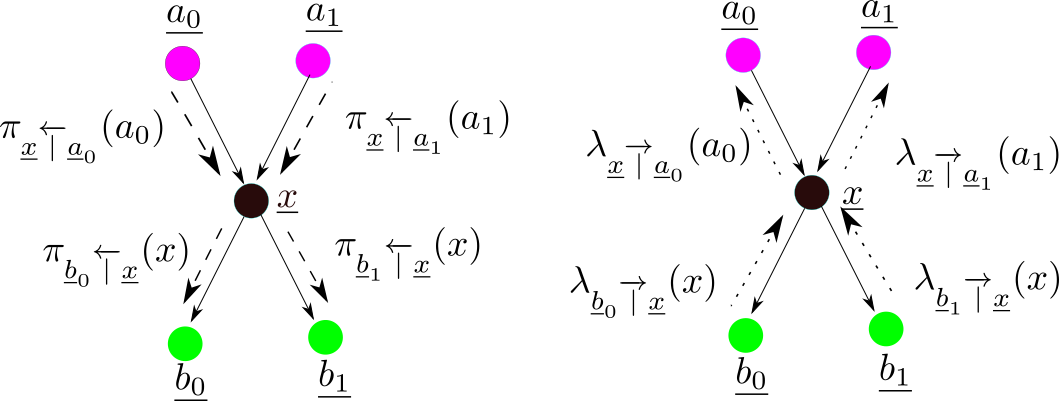
\includegraphics[width=6in]{mpass/pi-lam.png}
\caption{Node $\rvx$ receiving
and sending messages to
 its neighbors. (neighbors=
parents and children).
}
\label{fig-pi-lam}
\end{figure}


We define a {\bf memory matrix}
$\calm_{\rvx}$ for node $\rvx$
as

\beq
\calm_{\rvx}=
[
\calm^+_{\rvx},
\calm^-_{\rvx}]
\;,
\eeq
where $+=$future, $-=$past, and 

\beq
\calm^+_{ \rvx}=
\left[
\begin{array}{cc}
\pi_{\rvb\ldart\rvx}(\cdot)
&
\lam_{\rvb\rdart\rvx}(\cdot)
\end{array}
\right]_{\rvb\in ch(\rvx)}
=[\calm^+_{\rvb, \rvx}]_{\rvb\in ch(\rvx)}
\;,
\eeq

\beq
\calm^-_{\rvx}=
\left[
\begin{array}{c}
\pi_{\rvx\ldart\rva}(\cdot)
\\
\lam_{\rvx\rdart\rva}(\cdot)
\end{array}
\right]_{\rva\in  pa(\rvx)}
=[\calm^-_{\rvx, \rva}]_{\rva\in pa(\rvx)}
\;.
\eeq 
Note that

\beq
\calm^-_{\rvx, \rva}=
\calm^+_{\rva, \rvx}
\label{eq-mem-overlap-poly}
\eeq
for every arrow $\rvx\larrow\rva$.
We will refer to
Eqs.(\ref{eq-mem-overlap-poly}) as
the {\bf memory overlap
conditions}.

We will also use a permuted version of the 
memory matrix

\beq
\calm'_{\rvx}=
[
\calm^{OUT}_{\rvx},
\calm^{IN}_{\rvx}]
\;,
\eeq
where

\beq
\calm^{OUT}_{ \rvx}=
\left(
\begin{array}{c}
[\pi_{\rvb\ldart\rvx}(\cdot)]_
{\rvb\in ch(\rvx)}
\\
{[}\lam_{\rvx\rdart\rva}(\cdot)]_
{\rva\in  pa(\rvx)}\;,
\end{array}
\right)
\\
=
[\calm^{OUT}_{\rvx,\rvn}]_{\rvn\in nb(\rvx)}
\;, 
\eeq

\beq
\calm^{IN}_{\rvx}=
\left(
\begin{array}{c}
[\pi_{\rvx\ldart\rva}(\cdot)]_
{\rva\in  pa(\rvx)}
\\
{[}\lam_{\rvb\rdart\rvx}(\cdot)]_
{\rvb\in ch(\rvx)}
\end{array}
\right)
\\
=
[\calm^{IN}_{\rvx,\rvn}]_{\rvn\in nb(\rvx)}
\;.
\eeq


\hrule

For times $t=0, 1, \dots, T-1$,
 we calculate $\calm^{(t)}_\rvx$ in
two steps: first we calculate $\calm^{(t)IN}_\rvx$
from earlier memories at time $t-1$,
 then
we calculate $\calm^{(t)OUT}_\rvx$:

\begin{figure}[h!]
\centering
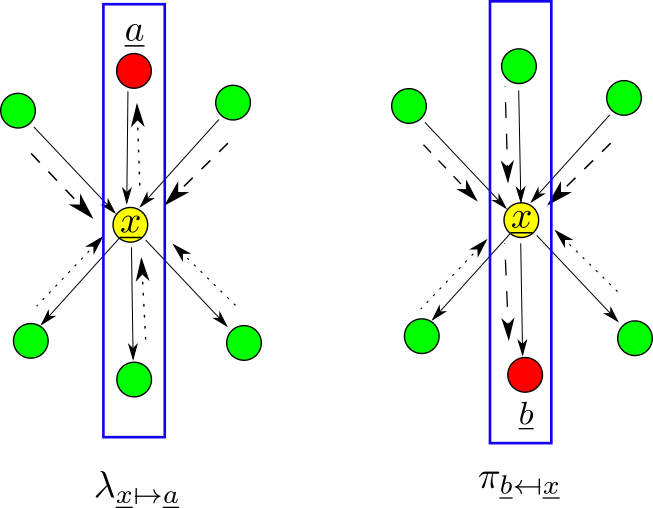
\includegraphics[width=3.5in]
{mpass/mpass-messages.png}
\caption{
Subgraph of a bnet
showing two cases (RULE 1
 and RULE 2)
of message info flow.
The yellow
node is a gossip monger.
It receives messages from
all the green nodes,
and then it relays a joint
message to the red node.
Union of green nodes and the red node = full
 neighborhood of yellow node.
There are two possible
cases: the
red node is either a parent
or a child of the yellow
one. As usual, we use arrows with
dashed (resp., dotted) shafts for
downstream (resp., upstream) messages. 
Blue boxes indicate Markov chain case. }
\label{fig-messages-gen}
\end{figure}

An {\bf evidence node} is a
node whose TPM is a delta function
set to a particular state of the node. 
We will assume, without loss of generality,
that all evidence nodes are leaf nodes.
If that is not the case, 
any
evidence node $\rve$
that is not
a leaf node,
can be given a new
companion leaf node $\rvl$
connected to $\rve$ by 
an arrow $\rvl\larrow \rve$,
and such that
$\rvl$ has a delta
function TPM.



\begin{enumerate}
\item {\bf Calculating
$\calm^{(t)IN}_\rvx$
from signals received from
 $\rvn\in nb(\rvx)$, sent at earlier time $t-1$:}

Set

\beq
\calm^{(t)-}_{\rvx, \rva}|_\pi=
\calm^{(t-1)+}_{\rva, \rvx}|_\pi
\;,
\eeq
for all $\rva\in pa(\rvx)$,
and 
\beq
\calm^{(t)+}_{\rvb, \rvx}|_\lam=
\calm^{(t-1)-}_{\rvx, \rvb}|_\lam
\;,
\eeq
for all $\rvb\in ch(\rvx)$.
By $X|_\lam$ (resp., $X|_\pi$)
we mean the $\lam$ (resp., $\pi$)
component of $X$.

\item {\bf Calculating $\calm^{(t)OUT}_\rvx$
from already calculated $\calm^{(t)IN}_\rvx$:}

Let $\rva^{na}=
(\rva_i)_{i=0, 1, \ldots, na-1}$
denote the parents of $\rvx$
and
$\rvb^{nb}=
(\rvb_i)_{i=0, 1, \ldots, nb-1}$
its children.

Define

\beqa
\label{eq-mp-pix}
\pi_\rvx(x)&=&
\sum_{a^{na}} P(x|a^{na})
\prod_i
\pi_{\rvx\ldart\rva_i}
(a_i)\\
&=&E_{\rva^{na}}[P(x|a^{na})]
\eeqa
(boundary case: if $\rvx$
is a root node, use $\pi_\rvx(x)=P(x)$.)
and

\beq
\lam_\rvx(x)=
\prod_i
\lam_{\rvb_i\rdart \rvx}(x)
\;.
\label{eq-mp-lamx}
\eeq
(boundary case: if $\rvx$
is a leaf node, use $\lam_\rvx(x)=1$.)
\begin{itemize}

\item{\bf RULE 1: (red parent)}

From
the $\lam_{\rvx \rdart\rva}$
panel of Fig.\ref{fig-messages-gen},
 we get

\begin{align}
\label{eq-mp-rule1}
\underbrace{\lam_{\rvx\rdart\rva_i}
(a_i)}_{OUT}&=
\caln(!a_i)
\sum_x\left[
\underbrace{\lam_\rvx(x)}_{IN}
\sum_{(a_k)_{k\neq i}}\left(
P(x|a^{na})\prod_{k\neq i}
\underbrace{\pi_
{\rvx\ldart\rva_k}
(a_k)}_{IN}
\right)\right]
\\&=
\caln(!a_i)
\sum_x\left[
\lam_\rvx(x)
E_{(\rva_k)_{k\neq i}}[P(x|a^{na})]\right]
\\&=
\caln(!a_i)
E_{(\rva_k)_{k\neq i}}E_{\rvx|a^{na}}
\lam_\rvx(x)
\end{align}
(boundary case:
if $\rvx$ is a root node, use
$\lam_{\rvx\rdart\rva_i}
(a_i)=\caln(!a_i)$.)

\item{\bf RULE 2: (red child)}

From the $\pi_{\rvb \ldart\rvx}$
panel of
Fig.\ref{fig-messages-gen},
we get


\beq
\underbrace{\pi_{\rvb_i\ldart\rvx}
(x)}_{OUT}=
\caln(!x)
\underbrace{\pi_\rvx(x)}_{IN}
\prod_{k\neq i}
\underbrace{\lam_{\rvb_k\rdart \rvx}(x)}_{IN}
\label{eq-mp-rule2}
\eeq
(boundary case:
if $\rvx$ is a leaf node, use
$\pi_{\rvb_i\ldart\rvx}(x)=
\caln(!x)\pi_\rvx(x)$
.)

\end{itemize}
\end{enumerate}
In the above
equations, if the
range set of a product is empty, then
 define the product as 1; i.e.,
$\prod_{k\in \emptyset}F(k)=1$.


\hrule\noindent
{\bf Claim:} Define

\beq
BEL^{(t)}(x)=\caln(!x)
\lam^{(t)}_\rvx(x)
\pi^{(t)}_\rvx(x)
\;.\eeq
Then

\beq
\lim_{t\rarrow \infty}BEL^{(t)}(x)=P(x|\eps)
\;.
\eeq
This  says that
the belief in $\rvx=x$
converges to $P(x|\eps)$ and it
equals the product
of messages received from all
parents and children of $\rvx=x$.

\subsection{How BP algo
for polytrees reduces to the 
BP algo for Markov chains}

It is instructive
to see
how the
BP algo
for polytrees reduces to 
BP algo for Markov chains.

For a Markov chain, node
$\rvx$ has a single parent (i.e., ancestor) $\rva$
and a single child $\rvb$.

Therefore, 
Eqs.(\ref{eq-mp-pix}) and (\ref{eq-mp-lamx}) reduce to

\beq
\pi_\rvx(x)=
\sum_a
P(x|a)\pi_{\rvx\ldart\rva}(a)
\eeq
and

\beq
\lam_\rvx(x)=
\lam_{\rvb\rdart \rvx}(x)
\;.
\eeq

RULE 1 given by Eq.(\ref{eq-mp-rule1}) reduces to

\beqa
\lam_{\rvx\rdart \rva}(a)
&=&
\caln(!a)\sum_x
\lam_\rvx(x)P(x|a) 
\\
&=&
\caln(!a)\sum_x
\lam_{\rvb\rdart \rvx}(x)P(x|a) 
\eeqa

RULE 2 given by Eq.(\ref{eq-mp-rule2}) reduces to

\beqa
\pi_{\rvb\ldart \rvx}(x)
&=&
\caln(!x)\pi_\rvx(x)
\\
&=&
\sum_a
P(x|a)\pi_{\rvx\ldart\rva}(a)
\;.
\eeqa



\section{Derivation of BP Algorithm
for Polytrees}

This derivation is taken from
 the 1988 book Ref.\cite{pearl-1988book}
by Judea Pearl, where it
is presented very lucidly. We only
made some minor
changes in notation.

\hrule\noindent
 {\bf Notation}

The BP algorithm yields an expansion
 for $P(x|\eps)$.

$\rvx$= the focus node,
arbitrary node of bnet that we are
focusing on to calculate its $P(x|\eps)$.



$(\rva_i)_{i=0,1, \ldots, na-1}$. = parent nodes
 (mnemonic: a=ancestor) of $\rvx$

$(\rvb_i)_{i=0,1, \ldots, nb-1}$. =
children nodes of $\rvx$.

$\rveps$= set of nodes for which
 there is evidence; that is,
$\rveps=\eps$, so
the state of these nodes is fixed.


$\rveps^-_\rvx= \rveps\cap an(\rvx)$
(evidence in past of $\rvx$)\footnote{
Careful:
Chapter 4
of Ref.\cite{pearl-1988book}
uses $-$ indicate the future
and $+$ to indicate
 the past. This
is the opposite of our notation.}

$\eps^-_{\rvx \rva_i}=
\eps^-_{\rvx}\cap an(\rva_i)$.

Note that $\eps^-_\rvx=\cup_i 
\eps^-_{\rvx \rva_i}$

$\rveps^+_\rvx= \rveps\cap [de(\rvx)\cup\rvx]$
(evidence in future of $\rvx$)

$\eps^+_{\rvx \rvb_i}=
\eps^+_{\rvx}\cap
 [de(\rvb_i)\cup \rvb_i]$.

Note that $\eps^+_\rvx=\cup_i 
\eps^+_{\rvx \rvb_i}$

Note that $\rveps=\rveps^+_\rvx \cup \eps^-_\rvx$

\beq
\pi_{ \rvx}(x)
=
P(x|\eps^-_\rvx)
\eeq

\beq
\pi_{ \rvx\ldart\rva_i}(a_i)=
P(a_i|\eps^-_{\rvx \rva_i})
\eeq

\beq
\pi_{ \rvb_i\ldart\rvx}(x)=
P(x|\eps^-_{\rvx \rvb_i})
\eeq

\beq
\lam_{\rvx} (x)=P(\eps^+_\rvx|x)
\eeq

\beq
\lam_{\rvb_i\rdart \rvx} (x)=
P(\eps^+_{\rvx \rvb_i}|x)
\eeq

\beq
\lam_{\rvx\rdart \rva_i} (a_i)=
P(\eps^+_{\rvx \rva_i}|a_i)
\eeq


\hrule\noindent
{\bf Expansions
of $\lam_\rvx(x)$ and $\pi_\rvx(x)$
into products of single node messages.}

\beqa
\underbrace{
P(x|\eps^-_\rvx)
}_{\pi_\rvx(x)}
&=&
P(x|\cup_i \eps^-_{\rvx \rva_i})
\\
&=&
\sum_{a^{na}}
P(x|a^{na})
P( a^{na}|\cup_i \eps^-_{\rvx \rva_i})
\\
&=&
\sum_{a^{na}}
P(x|a^{na})
\prod_i
\underbrace{
P(a_i| \eps^-_{\rvx \rva_i})}_{
\pi_{\rvx\ldart \rva_i}(a_i)
}
\eeqa

\beq
\underbrace{
P(\eps^+_\rvx|x)
}_{\lam_\rvx(x)}
=\prod_i
\underbrace{
P(\eps^+_{\rvx \rvb_i}|x)
}_{\lam_{\rvb_i\rdart \rvx}(x)}
\eeq
\hrule

Note that past and future evidences
$\eps^-_\rvx$ and $\eps^+_\rvx$
that are
causally connected to $\rvx$
are
conditionally
independent at fixed $\rvx$:

\beq
P(\eps^+_\rvx, \eps^-_\rvx|x)
=
P(\eps^+_\rvx|x) P(\eps^-_\rvx|x)
\;.
\eeq

This observation is key to the proof of
the following claim:

\begin{claim}
\beqa
P(x| \eps^+_\rvx, \eps^-_\rvx)
&=&
P(\eps^+_\rvx|x) P(x|\eps^-_\rvx
)\frac{1}{P(\eps^+_\rvx|\eps^-_\rvx)}
\\
&=&
\caln(!x)
P(\eps^+_\rvx|x)P(x|\eps^-_\rvx)
\\
&=&
\caln(!x)\;\;\;
(\eps^+_\rvx\larrow x \larrow \eps^-_\rvx)
\\&=&
\caln(!x)
\lam_\rvx (x)
\pi_\rvx(x)
\eeqa


\end{claim}
\proof

\beqa
 P(x|\eps^+_\rvx, \eps^-_\rvx)
&=&
P(\eps^+_\rvx, \eps^-_\rvx|x)\frac{P(x)}{P(\eps^+_\rvx, \eps^-_\rvx)}
\\
&=&
P(\eps^+_\rvx|x) P(\eps^-_\rvx|x)\frac{P(x)}{P(\eps^+_\rvx, \eps^-_\rvx)}
\\
&=&
P(\eps^+_\rvx|x) P(x|\eps^-_\rvx
)\frac{P(\eps^-_\rvx)}{P(\eps^+_\rvx, \eps^-_\rvx)}
\\
&=&
P(\eps^+_\rvx|x) P(x|\eps^-_\rvx
)\frac{1}{P(\eps^+_\rvx|\eps^-_\rvx)}
\eeqa
\qed

Next we prove BP rules 1 and 2.

\begin{itemize}
\item {\bf RULE 1 (red parent)}

\begin{figure}[h!]
\centering
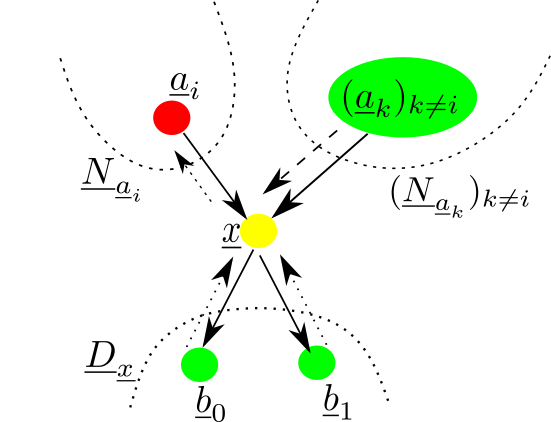
\includegraphics[width=2.65in]
{mpass/mpass-rule-1.png}
\caption{This figure is
used in the derivation of the BP
RULE 1.}
\label{fig-mpass-rule-1}
\end{figure}

Note that

\beqa
\eps^+_\rvx \cup \cup_{k\neq i}\eps^-_{\rvx \rva_k}
&=&
(\eps^+_\rvx\cup \eps^-_\rvx) - \eps^-_{\rvx \rva_i}
\\
&=&
\eps^+_{\rvx \rva_i}
\eeqa

Let $y=(a_k)_{k\neq i}$ and
$\eps^-_\rvy=(\eps^-_{\rvx \rva_k})_{k\neq i}$.

\beqa
\underbrace{
P(\eps^+_{\rvx \rva_i}|a_i)
}_{\lam_{\rvx\rdart\rva_i}(a_i)}
&=&
P(\eps^+_\rvx, \eps^-_\rvy|a_i)
\\
&=&
\sum_x
\sum_y
P(\eps^+_\rvx, \eps^-_\rvy|x,y)
P(x, y|a_i)
\\
&=&
\sum_x
\sum_y
P(\eps^+_\rvx|x)
P(\eps^-_\rvy|y)
P(x|y, a_i )P(y|a_i)
\\
&=&
P(\eps^-_\rvy)
\sum_x
\sum_y
P(\eps^+_\rvx|x)
\frac{P(y|\eps^-_\rvy)}{P(y)}
P(x|y, a_i )
\underbrace{P(y|a_i)}_{=P(y)}
\\
&=&
\caln(!a_i)
\sum_x
\sum_y
P(\eps^+_\rvx|x)
P(x|
\underbrace{
y, a_i
}_{a^{na}}
)P(y|\eps^-_\rvy)
\\
&=&
\caln(!a_i)
\sum_x
\underbrace{
P(\eps^+_\rvx|x)
}_{\lam_{\rvx}(x)}
\sum_{(a_k)_{k\neq i}}
P(x| a^{na})
\prod_{k\neq i}
\underbrace{
P(a_k|\eps^-_{\rvx \rva_k})
}_{\pi_{\rvx\ldart \rva_k}(a_k)}
\eeqa

\item{\bf RULE 2 (red child)}

\begin{figure}[h!]
\centering
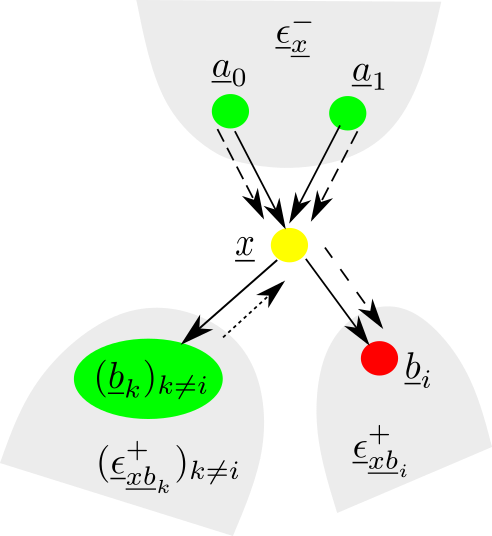
\includegraphics[width=2.5in]
{mpass/mpass-rule-2.png}
\caption{This figure is
used in the derivation of the BP
RULE 2.}
\label{fig-mpass-rule-2}
\end{figure}

Note that

\beqa
(\cup _{k\neq i}
\eps^+_{\rvx \rvb_k})\cup \eps^-_\rvx
&=&
(\eps^+_\rvx\cup \eps^-_\rvx) - \eps^+_{\rvx \rvb_i}
\\
&=&
\eps^-_{\rvx \rvb_i}
\eeqa


\beqa
\underbrace{
P(x| \eps^-_{\rvx \rvb_i})
}_{\pi_{\rvb_i\ldart \rvx}(x)}
&=&
P(x| (\eps^+_{\rvx \rvb_k})_{k\neq i}, \eps^-_\rvx)
\\
&=&
\caln(!x)
P((\eps^+_{\rvx \rvb_k})_{k\neq i}|x)P(x|\eps^-_\rvx)
\\&=&
\caln(!x)
\left(
\prod_{k\neq i}
\underbrace{
P(\eps^+_{\rvx \rvb_k}|x)
}_{\lam_{\rvb_k\rdart\rvx}(x)}
\right)
\underbrace{
P(x|\eps^-_\rvx)
}_{\pi_\rvx(x)}
\eeqa

\end{itemize}


\section{Example of BP algo for a  Tree}

In this section, we 
describe how to apply
the BP algo
to the tree bnet Fig.\ref{fig-mp-9tree}.
In Fig.\ref{fig-mp-9tree}, if we 
replace each integer $i$ by 
the random variable $\rvA_i$,
we get an {\bf original bnet}, 
and if we replace each
$i$
by $\ucalm_{\rvA_i}$,
we get the {\bf BP memory bnet}
of the original bnet.
In Fig.\ref{fig-mp-9tree},
the magenta  nodes are evidence nodes
and the green ones aren't.

We want to solve for the 
memory matrices of the 
memory bnet. To do so,
we use the {\bf BP dynamic bnet}
Fig.\ref{fig-propagation-9tree}.
The steps encoded
in the dynamic bnet 
are shown in Fig.\ref{fig-multiframe-9tree}.
Fig.\ref{fig-multiframe-9tree}
has frames in chronological order,
showing the direction of travel
of the $\pi\&\lam$ information. 
This sequence of frames also indicates 
the order
in which we solve for the entries of
 the memory matrices.
The information first emanates from the evidence nodes.
It propagates generally upstream,
although some nodes
can generate downstream flow. Some of the 
info  reaches the root node and is  reflected there.
The root node is the only one that 
is capable of reflection (i.e., instant output
along an arrow, 
in response to input along that arrow).
Eventually, all info
reaches the leaf nodes 
via downstream propagation and is absorbed there.


\begin{figure}[h!]
\centering
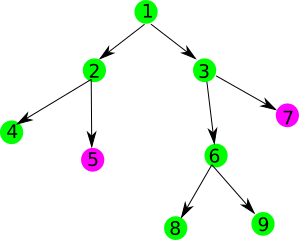
\includegraphics[width=2.5in]
{mpass/mp-9tree.png}
\caption{Example tree bnet
used to illustrate BP.
} 
\label{fig-mp-9tree}
\end{figure}



\begin{figure}[h!]
$$\xymatrix{
\rvA_1 
&\ucalm^{(0)}_{\rvA_1}\ar[r]
&\ucalm^{(1)}_{\rvA_1}\ar[r]
&\ucalm^{(2)}_{\rvA_1}\ar[r]\ar[dr]\ar[ddr]
&\ucalm^{(3)}_{\rvA_1}\ar[r]
&\ucalm^{(4)}_{\rvA_1}\ar[r]
&\ucalm^{(5)}_{\rvA_1}
\\
\rvA_2 
&\ucalm^{(0)}_{\rvA_2}\ar[r]
&\ucalm^{(1)}_{\rvA_2}\ar[r]\ar[ur]\ar[ddr]
&\ucalm^{(2)}_{\rvA_2}\ar[r]
&\ucalm^{(3)}_{\rvA_2}\ar[r]\ar[ddr]\ar[dddr]
&\ucalm^{(4)}_{\rvA_2}\ar[r]
&\ucalm^{(5)}_{\rvA_2}
\\
\rvA_3 
&\ucalm^{(0)}_{\rvA_3}\ar[r]
&\ucalm^{(1)}_{\rvA_3}\ar[r]\ar[uur]\ar[dddr]
&\ucalm^{(2)}_{\rvA_3}\ar[r]
&\ucalm^{(3)}_{\rvA_3}\ar[r]\ar[dddr]\ar[ddddr]
&\ucalm^{(4)}_{\rvA_3}\ar[r]
&\ucalm^{(5)}_{\rvA_3}
\\
\rvA_4 
&\ucalm^{(0)}_{\rvA_4}\ar[r]
&\ucalm^{(1)}_{\rvA_4}\ar[r]
&\ucalm^{(2)}_{\rvA_4}\ar[r]
&\ucalm^{(3)}_{\rvA_4}\ar[r]
&\ucalm^{(4)}_{\rvA_4}\ar[r]
&\ucalm^{(5)}_{\rvA_4}
\\
\rvA_5 
&\ucalm^{(0)}_{\rvA_5}\ar[r]\ar[uuur]
&\ucalm^{(1)}_{\rvA_5}\ar[r]
&\ucalm^{(2)}_{\rvA_5}\ar[r]
&\ucalm^{(3)}_{\rvA_5}\ar[r]
&\ucalm^{(4)}_{\rvA_5}\ar[r]
&\ucalm^{(5)}_{\rvA_5}
\\
\rvA_6 
&\ucalm^{(0)}_{\rvA_6}\ar[r]
&\ucalm^{(1)}_{\rvA_6}\ar[r]
&\ucalm^{(2)}_{\rvA_6}\ar[r]\ar[ddr]\ar[dddr]
&\ucalm^{(3)}_{\rvA_6}\ar[r]
&\ucalm^{(4)}_{\rvA_6}\ar[r]\ar[ddr]\ar[dddr]
&\ucalm^{(5)}_{\rvA_6}
\\
\rvA_7 
&\ucalm^{(0)}_{\rvA_7}\ar[r]\ar[uuuur]
&\ucalm^{(1)}_{\rvA_7}\ar[r]
&\ucalm^{(2)}_{\rvA_7}\ar[r]
&\ucalm^{(3)}_{\rvA_7}\ar[r]
&\ucalm^{(4)}_{\rvA_7}\ar[r]
&\ucalm^{(5)}_{\rvA_7}
\\
\rvA_8 
&\ucalm^{(0)}_{\rvA_8}\ar[r]
&\ucalm^{(1)}_{\rvA_8}\ar[r]
&\ucalm^{(2)}_{\rvA_8}\ar[r]
&\ucalm^{(3)}_{\rvA_8}\ar[r]
&\ucalm^{(4)}_{\rvA_8}\ar[r]
&\ucalm^{(5)}_{\rvA_8}
\\
\rvA_9 
&\ucalm^{(0)}_{\rvA_9}\ar[r]
&\ucalm^{(1)}_{\rvA_9}\ar[r]
&\ucalm^{(2)}_{\rvA_9}\ar[r]
&\ucalm^{(3)}_{\rvA_9}\ar[r]
&\ucalm^{(4)}_{\rvA_9}\ar[r]
&\ucalm^{(5)}_{\rvA_9}
\\
}$$
\caption{BP dynamic bnet for the bnet
Fig.\ref{fig-mp-9tree}.}
\label{fig-propagation-9tree}
\end{figure}

\begin{figure}[h!]
\centering
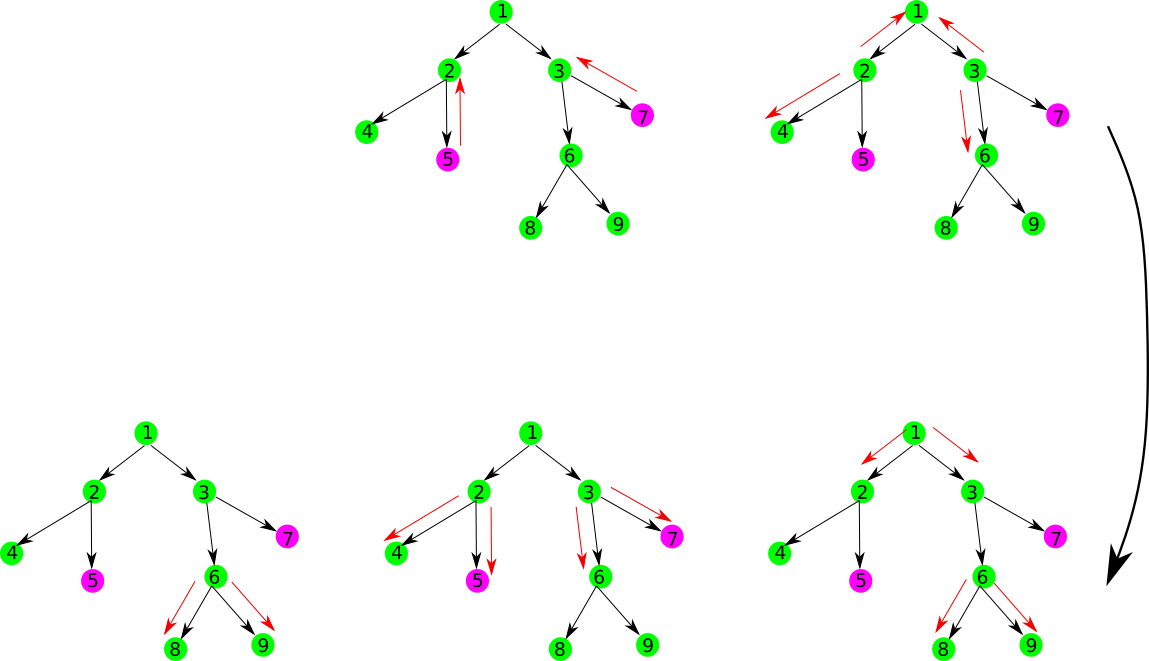
\includegraphics[width=7in]
{mpass/mp-multiframe-9tree.png}
\caption{Steps encoded in
the bnet 
Fig.\ref{fig-propagation-9tree}.
} 
\label{fig-multiframe-9tree}
\end{figure}

\clearpage
\newpage
\section{Bipartite bnets}

By a {\bf bipartite bnet}
we will mean a bnet
in which all nodes
are either root nodes (parentless)
or leaf nodes (childless).
BP
simplifies when dealing with
bipartite bnets. In this section,
we will explain how
it simplifies. But
before doing so,
let us explain how the
following two types of
diagrams
can be replaced by
equivalent bipartite bnets:

\begin{itemize}
\item Factor Graphs
\item Tree bnets
\end{itemize}
\hrule

Consider a product $g=\prod_\alp f_\alp$
of scalar functions
 $f_\alp:S_{\rvx_0}
\times S_{\rvx_1}
\times \ldots S_{\rvx_{nx-1}}\rarrow \RR$
for $\alp=0, 1, \ldots, nf-1$. For instance,
consider $g:S_{\rvx_0}
\times S_{\rvx_1} \times S_{\rvx_2}\rarrow \RR$
defined by:

\beq
g(x_0,x_1,x_2) = f_0(x_0)
f_1(x_0,x_1)f_2(x_0,x_1)f_3(x_1,x_2)
\label{eq-g-fun}
\;.
\eeq
The {\bf factor graph}
for this function $g$
 is given by Fig.\ref{fig-fac-graph}.


\begin{figure}[h!]
\centering
$$\xymatrix{
*++[o][F]{x_0}\ar@{-}[d]\ar@{-}[dr]\ar@{-}[drr]
&*++[o][F]{x_1}\ar@{-}[d]\ar@{-}[dr]\ar@{-}[drr]
&*++[o][F]{x_2}\ar@{-}[dr]
\\
*+[F]{f_0}
&*+[F]{f_1}
&*+[F]{f_2}
&*+[F]{f_3}
}$$
\caption{Factor graph for function
$g$ defined by Eq.(\ref{eq-g-fun}).}
\label{fig-fac-graph}
\end{figure}

\begin{figure}[h!]
\centering
$$\xymatrix{
\rvx_0\ar[d]\ar[dr]\ar[drr]
&\rvx_1\ar[d]\ar[dr]\ar[drr]
&\rvx_2\ar[dr]
\\
\rvf_0&\rvf_1&\rvf_2&\rvf_3
}$$
\caption{Bipartite bnet
corresponding to factor
graph Fig.\ref{fig-fac-graph}.}
\label{fig-bip-bnet}
\end{figure}

One
can map
any factor graph (the ``source")
to a special bipartite bnet (the ``image"),
as follows.
Replace each $x_i$ by $\rvx_i\in S_{\rvx_i}$
for $i=0,1, \ldots, nx-1$
 and each
 $f_\alpha$ by $\rvf_\alpha$
for $\alpha=0, 1, \ldots, nf-1$.
Then replace
the connections (edges)
of the factor graph
by arrows from $\rvx_i$ to
$\rvf_\alpha$. For example,
Fig.\ref{fig-bip-bnet}
is the image bipartite bnet of the source factor
graph Fig.\ref{fig-fac-graph}.


Let $\rvx^{nx}=
(\rvx_0, \rvx_1, \ldots, \rvx_{nx-1})$
and
$\rvf^{nf}=
(\rvf_0, \rvf_1, \ldots, \rvf_{nf-1})$.
Let\footnote{
Note that we are using
$f_\alpha$
to denote both a function
$f_\alp(\cdot)$  and a boolean
value. Which one we mean
will be clear from context.
$f_\alp$ could also be used to
denote, besides a function and a boolean value,
the real number
$y_\alp=f_\alpha(x_{nb(\rvf_\alpha)})$.
However, we won't be using it that third way
in this chapter.}
$f_\alp\in \bool$ for all $\alp$,
and $y_\alp=
f_\alpha(x_{nb(\rvf_\alpha)})$.
Here we are using $nb(\rvf_\alp)$
to denote  the neighborhood
of node $\rvf_\alp$
in the image bipartite bnet,
and we are using $x_S$ to denote
$(x_i)_{i\in S}$.
Without loss of
generality,
we will assume
that $y_\alp\in[0,1]$ for all $\alp$.
Then we define the node TPMs, printed
in blue, for the
image bipartite bnet, 
as follows.




\beq\color{blue}
P(f_\alpha|x_{nx(\rvf_\alpha)})=
y_\alp
\delta(f_\alp, 1)
+
[1-y_\alp]
\delta(f_\alp, 0)
\;
\eeq
for $\alp=0, 1, \ldots , nf-1$
and

\beq\color{blue}
P_{\rvx_i}(x_i)= \text{arbitrary prior}
\eeq
for $i=0, 1, \ldots, nx-1$.

Note that

\beq
P(f^{nf}=1^{nf}|x^{nx})=
\prod_\alpha
f_\alpha(x_{nb(\rvf_\alpha)})
\;.
\eeq

\hrule
A {\bf tree bnet}
is a bnet for which all
nodes have exactly
one parent except
for the apex root
node which has none.
A tree bnet
is very much like
the filing system
in a computer.

One can map a tree
 bnet (the ``source")
into
an equivalent
bipartite bnet (the ``image") as follows.
Replace
each arrow

\beq
\xymatrix{
\rvx\ar[rr]&&\rvy
}
\eeq
of the tree bnet by


\beq
\xymatrix{
\rvx\ar[r]
&
\ul{P_{\rvy|\rvx}}
&
\rvy\ar[l]
}\;.
\eeq
For example,
the tree bnet Fig.\ref{fig-part3-tree}
has the image
bipartite bnet given by
Fig.\ref{fig-part3-tree-junc-tree}.
The
bnet Fig.\ref{fig-part3-tree-bip-bnet}
is just
a different
way of drawing the bnet
Fig.\ref{fig-part3-tree-junc-tree}.

\begin{figure}[h!]
$$\xymatrix{
\rvA\ar[d]\ar[rrd]
\\
\rvA_0\ar[d]\ar[rd]&&\rvA_1
\\
\rvA_{00}&\rvA_{01}
}
$$
\caption{Example of a tree bnet.}
\label{fig-part3-tree}
\end{figure}


\begin{figure}[h!]
$$\xymatrix{
\rvA\ar[d]\ar[rrd]
\\
\ul{P_{\rvA_0|\rvA}}&&\ul{P_{\rvA_1|\rvA}}
\\
\rvA_0\ar[u]\ar[d]\ar[rd]&&\rvA_1\ar[u]
\\
\ul{P_{\rvA_{00}|\rvA_0}}&\ul{P_{\rvA_{01}|\rvA_0}}
\\
\rvA_{00}\ar[u]&\rvA_{01}\ar[u]
}
$$
\caption{Bipartite bnet
corresponding
to tree bnet Fig.\ref{fig-part3-tree}.}
\label{fig-part3-tree-junc-tree}
\end{figure}

\begin{figure}[h!]
\centering
$$\xymatrix{
\rvA\ar[dr]\ar[drr]
&\rvA_{0}\ar[d]\ar[drr]\ar[drrr]
&\rvA_{1}\ar[d]
&\rvA_{00}\ar[d]
&\rvA_{01}\ar[d]
\\
&\ul{P_{\rvA_{0}|\rvA}}
&\ul{P_{\rvA_{1}|\rvA}}
&\ul{P_{\rvA_{00}|\rvA_0}}
&\ul{P_{\rvA_{01}|\rvA_0}}
}$$
\caption{
Different
way of drawing
the bnet Fig.\ref{fig-part3-tree-junc-tree}.}
\label{fig-part3-tree-bip-bnet}
\end{figure}

The node  TPMs, printed in blue,
for the image bipartite bnet
Fig.\ref{fig-part3-tree-junc-tree},
are as follows. We express the
TPMs of the image bnet
in terms of the
TPMs of the source bnet
Fig.\ref{fig-part3-tree}. Let

\beq\color{blue}
P(P_{\rvy|\rvx}| x, y)=
P_{\rvy|\rvx}(y|x)
\delta(P_{\rvy|\rvx}, 1)
+
(1-P_{\rvy|\rvx}(y|x))
\delta(P_{\rvy|\rvx}, 0)
\eeq
for all the
leaf
nodes $\ul{P_{\rvy|\rvx}}\in \bool$ of the
image bipartite bnet.
Also, let

\beq\color{blue}
P_\rvy(y)= \text{arbitrary prior}
\;
\eeq
for all the root nodes 
$\rvy$ of the
image bipartite bnet
except when
$\rvy$ corresponds to
the root node $\rvA$
of the source tree bnet.
In that exceptional case,

\beq\color{blue}
P_\rvy(y)= P_\rvA(y)
\;.
\eeq


\section{BP for
bipartite bnets (BP-BB)}
For
a bipartite
bnet as defined above,
with
root nodes $\rvx_i$
and leaf nodes $\rvf_\alp$,
let


\beq
nb(i)=\{\alp: \rvf_\alpha\in
nb(\rvx_i)\}
\;,
\eeq

\beq
nb(\alpha)=\{i: \rvx_i\in
nb( \rvf_\alpha)\}
\;,
\eeq

\beq
m_{\alp\ldart i}
(x_i)
=
\pi_{\rvf_\alpha \ldart\rvx_i }
(x_i)
\;,
\eeq

\beq
m_{\alp\rdart i}
(x_i)
=
\lam_{\rvf_\alp\rdart \rvx_i}
(x_i)
\;,
\eeq


\begin{figure}[h!]
\centering
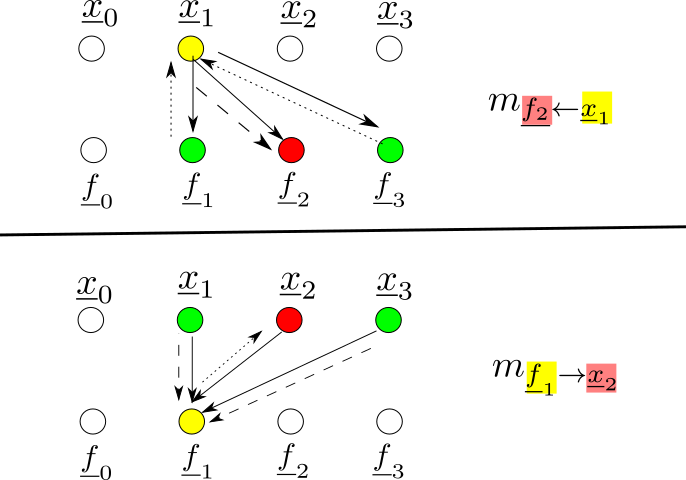
\includegraphics[width=3in]
{mpass/mpass-messages-bip.png}
\caption{
Fig.\ref{fig-messages-gen}
becomes this figure
for the special case of a
bipartite bnet. Union of green nodes and the red node = full
 neighborhood of yellow node.
There are two possible
cases:  the
red node is either a parent
or a child  of the yellow
node.}
\label{fig-messages-bip}
\end{figure}

Next we will
show how
to find $m_{\alp\ldart i}^{(t)}$
and $m_{\alp\rdart i}^{(t)}$
from 
$m_{\alp\ldart i}^{(t-1)}$
and $m_{\alp\rdart i}^{(t-1)}$.
\begin{enumerate}

\item {\bf
Traversing an $x$ (i.e., root) node.}

See
the
$m_{\rvf_2\ldart\rvx_2 }$ panel of
Fig.\ref{fig-messages-bip}.

For $i=0, 1, \ldots , nx-1$, if
 $\alp\in nb(i)$, then,

\beq
m^{(t)}_{\alp\ldart i }(x_i)
=
\prod_{
\beta\in nb(i)-\alpha}
m^{(t-1)}_{\beta\rdart i}(x_i)
\;,
\label{eq-mp-iter1}
\eeq
whereas if  $\alp\notin nb(i)$

\beq
m^{(t)}_{\alp\ldart i}(x_i)=
m^{(t-1)}_{\alp\ldart i}(x_i)
\;.
\eeq

\item {\bf
Traversing an $f$ (i.e., leaf) node.}

See the
$m_{\rvf_2\rdart \rvx_2}$ panel
of Fig.\ref{fig-messages-bip}.

For $\alp=0, 1, \ldots, nf-1$, if
 $i\in nb(\alp)$, then


\beqa
m^{(t)}_{\alp\rdart i}(x_i)
&=&
\sum_{(x_k)_{k\in nb(\alpha)-i}}
f_\alpha(x_{nb(\alpha)})
\prod_{k\in nb(\alpha)-i}
m^{(t-1)}_{\alp\ldart k }
(x_k)
\\
&=&
E^{(t-1)}_{(x_k)_{k\in nb(\alpha)-i}}[
f_\alpha(x_{nb(\alpha)})]
\;,
\label{eq-mp-iter2}
\eeqa
whereas if $i\notin nb(\alp)$

\beq
m^{(t)}_{\alp\rdart i}(x_i)
=
m^{(t-1)}_{\alp\rdart i}(x_i)
\;.
\eeq

\end{enumerate}

In the above
equations, if the
range set of a product is empty, then
 define the product as 1; i.e.,
$\prod_{k\in \emptyset}F(k)=1$.



\hrule\noindent
{\bf Claim:}

\beq
P(x_i|\eps)=
\lim_{t\rarrow
\infty}\caln(!x_i)\prod_{\alp\in nb(i)}
m^{(t)}_{\alp\rdart i}(x_i)
\;
\label{eq-m-prod}
\eeq
and

\beq
P(x_{nb(\alp)}|\eps)=\lim_{t\rarrow \infty}
\caln(!x_{nb(\alp)})
f_\alp(x_{nb(\alp)})
\prod_{k\in nb(\alp)}
m^{(t)}_{\alp\ldart k}(x_k)
\;.
\label{eq-f-m-prod}
\eeq


\subsection{BP-BB and general BP agree on Markov chains}

It is instructive to 
compare the belief values (i.e., $P(x_i|\eps)$)
obtained by
 applying the 
general (i.e., polytree)  BP  
and  BP-BB algorithms  to a Markov chain.
Next we show that both algorithms 
yield the same belief values.

\begin{figure}[h!]
$$
\begin{array}{cc}
\xymatrix{
&2\ar[dr]\ar[dl]\ar@[red]@{-->}@<-1ex>[dl]
\\
\beta
&&\alp\ar@[red]@{.>}@<-1ex>[ul]
}
&
\xymatrix{
&2\ar[dr]\ar[dl]\ar@[red]@{-->}@<1ex>[dr]
\\
\beta\ar@[red]@{.>}@<1ex>[ur]
&&\alp
}
\\
\\
(a)&(b)
\end{array}
$$
\caption{Traversing a root node of a Markov chain
(a)Propagation towards left (i.e., towards future).
(b)Propagation towards right (i.e., towards past).}
\label{fig-mp-markov-trans-root}
\end{figure}

Consider
the BP-BB rule for traversing a root node. 
When traveling
towards the left
as in Fig.\ref{fig-mp-markov-trans-root} (a), 
it implies that

\beq
m_{\alp \rdart 2}(x_2)= m_{\beta \ldart 2}(x_2)
\;,
\eeq
and
when traveling
towards the right
as in Fig.\ref{fig-mp-markov-trans-root} (b), 
it implies that

\beq
m_{\beta\rdart 2}(x_2)=m_{\alp\ldart 2}(x_2)
\;.
\eeq



\begin{figure}[h!]
$$
\begin{array}{cc}
\xymatrix{
3\ar[dr]
&&
2\ar[rd]\ar[dl]\ar@[red]@{-->}@<-1ex>[dl]
&&
1\ar[ld]\ar@[red]@{-->}@<1ex>[dl]
\\
&\beta
&&\alp\ar@[red]@{.>}@<-1ex>[ul]
}
&
\;\;\;\;\;
\xymatrix{
3\ar[dr]
&&
2\ar[rd]\ar[dl]\ar@[red]@{-->}@<1ex>[dr]
&&
1\ar[ld]
\\
&\beta\ar@[red]@{.>}@<1ex>[ur]
&&\alp\ar@[red]@{.>}@<-1ex>[ur]
}
\\
\\
(a)&(b)
\end{array}
$$
\caption{Traversing a leaf node of a Markov chain
(a)Propagation towards left (i.e., towards future).
(b)Propagation towards right (i.e., towards past).}
\label{fig-mp-markov-trans-leaf}
\end{figure}

Now consider the BP-BB rule for traversing a leaf node.
When
traveling to the left as
in Fig.\ref{fig-mp-markov-trans-leaf} (a),
it implies that

\beq
\underbrace{m_{\alp\rdart 2}(x_2)}_{\lam}
=
\sum_{x_1}
P(x_2|x_1) 
\underbrace{m_{\alp\ldart 1}(x_1)}_
{\pi}
\;.
\label{eq-markov-leaf-left}
\eeq
One can rewrite the
left and right
hand sides (LHS, RHS)
of Eq.(\ref{eq-markov-leaf-left})
as follows
 


\beq
RHS=
\sum_{x_1}
P(x_2|x_1) 
\pi_{\alp\ldart 1}(x_1)
\;,
\eeq
and

\beq
LHS=m_{\alp\rdart 2}(x_2)
=
m_{\beta\ldart 2}(x_2)
=
\pi_{\beta\ldart 2}(x_2)
\;,
\eeq
Therefore
 
\beq
\pi_{\beta\ldart 2}(x_2)
\sum_{x_1}
P(x_2|x_1) 
\pi_{\alp\ldart 1}(x_1)
\;.
\eeq


Once again, consider the BP-BB rule
 for traversing a leaf node.
When
traveling to the right as
in Fig.\ref{fig-mp-markov-trans-leaf} (b),
it implies that


\beq
\underbrace{m_{\alp\rdart1}(x_1)}_{\lam}
=
\sum_{x_2}
P(x_2|x_1) 
\underbrace{m_{\alp\ldart 2}(x_2)}_
{\pi}
\label{eq-markov-leaf-right}
\;.
\eeq
One can rewrite the
left and right
hand sides (LHS, RHS)
of Eq.(\ref{eq-markov-leaf-right})
as follows


\beqa
RHS=
&=&
\sum_{x_2}
P(x_2|x_1) 
\pi_{\alp\ldart 2}(x_2)
\\
&=&
\sum_{x_2}
P(x_2|x_1) 
\lam_{\beta\rdart 2}(x_2)
\;,
\eeqa
and

\beq
LHS=
\lam_{\alp\rdart 1}(x_1)
\;.
\eeq
Therefore,

\beq
\lam_{\alp\rdart 1}(x_1)=
\sum_{x_2}
P(x_2|x_1) 
\lam_{\beta\rdart 2}(x_2)
\;.
\eeq

Finally, note that Eq.(\ref{eq-m-prod}) becomes
\beqa
P(x_2|\eps)&=&
\caln(!x_2)
m_{\beta\rdart 2}(x_2)
m_{\alp\rdart 2}(x_2)
\\
&=&
\caln(!x_2)
m_{\alp\ldart 2}(x_2)
m_{\alp\rdart 2}(x_2)
\\
&=&
\caln(!x_2)
\pi_{\alp\ldart 2}(x_2)
\lam_{\alp\rdart 2}(x_2)
\\
&=&
\caln(!x_2)
P(x_2|\eps^-)
P(x_2|\eps^+)
\eeqa
and Eq.(\ref{eq-f-m-prod}) becomes

\beqa
P(x_2, x_1)
&=&
\caln(!x_2, !x_1)
P(x_2|x_1)
m_{\alp\ldart 1}(x_1)
m_{\alp\ldart 2}(x_2)
\\
&=&
\caln(!x_2, !x_1)
P(x_2|x_1)
\pi_{\alp\ldart 1}(x_1)
\pi_{\alp\ldart 2}(x_2)
\;.
\eeqa

\subsection{BP-BB and general BP 
agree on tree bnets.}

It is instructive to 
compare the belief values (i.e., $P(x_i|\eps)$)
obtained by
 applying the 
general (i.e., polytree)  BP  
and  BP-BB algorithms  to a tree bnet.
Next we show that both algorithms 
yield the same belief values.

\begin{figure}[h!]
\centering
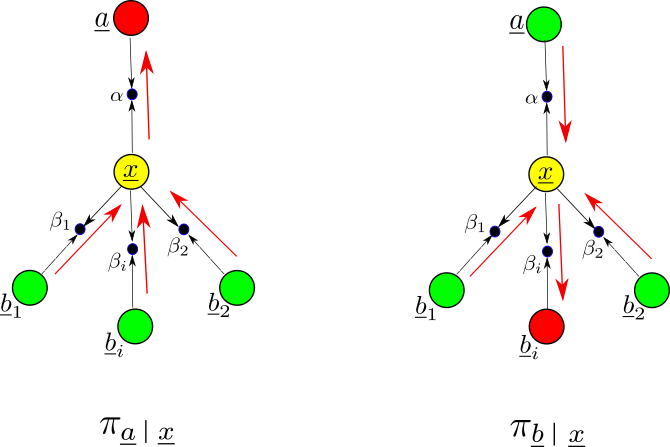
\includegraphics[width=4in]
{mpass/mpass-messages-bip-tree.png}
\caption{Subgraph of a tree bnet. 
This 
is the same as 
Fig.\ref{fig-messages-gen},
except that here the yellow
node has a single
parent because 
this is a subgraph of a tree
bnet, not
of an arbitrary
bnet like Fig.\ref{fig-messages-gen}.
The subgraph has been
converted to a subgraph
of a bipartite bnet
by inserting a collider leaf node, labeled
by a Greek letter, 
at the center
of each edge of the tree bnet.
Red arrows indicate
the direction
of message info flow.}
\label{fig-messages-bip-tree}
\end{figure}

Applying to the left panel of
Fig.\ref{fig-messages-bip-tree}
 the BP-BB rule
for traversing a root node, we get

\beq
m_{\alp\ldart \rvx}(x)=
\prod_{i}
m_{\beta_i\rdart \rvx}(x)
\;.
\label{eq-mp-tree-trans-x-rule1}
\eeq
Applying to the left panel of
Fig.\ref{fig-messages-bip-tree}
 the BP-BB rule
for traversing a leaf node, we get

\beq
m_{\alp\rdart\rva}(a)=
\caln(!a)
\sum_x
m_{\alp\ldart \rvx}(x)P(x|a)
\;.
\label{eq-mp-tree-trans-alp-rule1}
\eeq
Combining Eqs.(\ref{eq-mp-tree-trans-x-rule1})
and (\ref{eq-mp-tree-trans-alp-rule1}), we get

\beq
m_{\alp\rdart\rva}(a)=
\caln(!a)
\sum_x P(x|a)
\prod_{i}
m_{\beta_i\rdart \rvx}(x)
\;,
\eeq
which can be
rewritten as 

\beq
\lam_{\rvx\rdart\rva}(a)=
\caln(!a)
\sum_x P(x|a)
\underbrace{\prod_{i}
\lam_{\rvb_i\rdart \rvx}(x)}_
{\lam_\rvx(x)}
\;.
\label{eq-tree-rule1}
\eeq
Eq.\ref{eq-tree-rule1} is just RULE 1
for general BP.

Applying to the right panel of
Fig.\ref{fig-messages-bip-tree}
 the BP-BB rule
for traversing a root node, we get

\beq
m_{\beta_i\ldart \rvx}(x)=
\caln(!x)
m_{\alp\rdart \rvx}(x)
\prod_{k\neq i}m_{\beta_k\rdart\rvx}(x)
\label{eq-mp-tree-trans-x-rule2}
\eeq
Applying to the right panel of
Fig.\ref{fig-messages-bip-tree}
 the BP-BB rule
for traversing a leaf node, we get

\beqa
m_{\alp\rdart\rvx}(x)
&=&
\sum_a P(x|a) m_{\alp\ldart a}(a)
\\
&=&
\sum_a P(x|a) \pi_{\rvx\ldart a}(a)
\\
&=&
\pi_\rvx(x)
\label{eq-mp-tree-trans-alp-rule2}
\;.
\eeqa
Combining Eqs.(\ref{eq-mp-tree-trans-x-rule2})
and (\ref{eq-mp-tree-trans-alp-rule2}),
we get

\beq
\pi_{\rvb_i\ldart \rvx}(x)=
\caln(!x)
\pi_\rvx(x)
\prod_{k\neq i}\lam_{\rvb_k\rdart\rvx}(x)
\;.
\label{eq-tree-rule2}
\eeq
Eq.(\ref{eq-tree-rule2}) is just RULE 2
of general BP.




\section{BP-BB and sum-product decomposition}


BP-BB
yields what
is often
referred to as
a {\bf  sum-product decomposition}.
I don't like that name
because it is unnecessarily
confusing, and it fails to convey the
recursive nature\footnote{
By ``recursive nature",
we mean bootstraped definitions 
that lead to nested sums. 
The recursive nature 
of BP
is evident from 
RULES 1 and 2
that define $\lam$'s 
and $\pi$'s
in terms of other 
$\lam$'s and $\pi$'s.}
of the decomposition.
I prefer to call it a {\bf
recursive sum of products
(RSOP) decomposition},
and will call it so henceforth
in this chapter.

Expressing the marginals of a bnet
as RSOPs,
which is what BP does,
reduces the complexity
of the calculation.
(i.e.,
the total number
of additions
and multiplications
that need to be performed)
That makes
using the BP
algo very advantageous.
For instance, consider 
a Markov chain
$\rvx_{n-1}\larrow\cdots\larrow\rvx_1\larrow \rvx_0$,
where $x_i\in\{0,1,2\}$ for all $i$.
Note that if we calculate 
$P(x_{n-1})$ as follows

\beq
P(x_{n-1})=
\left[\sum_{x_{n-2}} P(x_{n-1}|x_{n-2})\ldots
\left[\sum_{x_1} P(x_2|x_1)
\left[\sum_{x_0}P(x_1|x_0)P(x_0)\right]\right]\ldots\right]
\;,
\eeq
we need to perform 
 $2(n-1)$ additions and $3(n-1)$ multiplications.
On the other hand, if we calculate $P(x_{n-1})$
as follows 

\beq
P(x_{n-1})=
\sum_{x_{n-2}} \ldots
\sum_{x_1} 
\sum_{x_0}
P(x_{n-1}|x_{n-2})
\ldots
P(x_2|x_1)
P(x_1|x_0)
P(x_0)
\;,
\eeq
we need to perform $3^n-1$ additions and
 $3^n(n-1)$
multiplications.

